% !TEX TS-program = xelatex
% !TEX encoding = UTF-8
% !Mode:: "TeX:UTF-8"

\documentclass[onecolumn,oneside]{SUSTechHomework}

\usepackage{float}

\author{胡玉斌}
\sid{11712121}
\title{Lab 5}
\coursecode{CS315}
\coursename{Computer Security}

\begin{document}
  \maketitle

  \section{Read the lab instructions above and finish all the tasks.}

  \section{Turn in the file name and entire smali method that you modified to write the username and password to the log from the Login App.}

    We modified \verb|LoginActivity.smali| file, and the smali method is \verb|attemptLogin()|.

    entire smali method that we modified:

    \begin{lstlisting}[language={java}]
      .method private attemptLogin()V
          .registers 9
      
          .prologue
          const/4 v7, 0x1
      
          const/4 v4, 0x0
      
          .line 147
          iget-object v5, p0, Ledu/wayne/securityclass/LoginActivity;->mAuthTask:Ledu/wayne/securityclass/LoginActivity$UserLoginTask;
      
          if-eqz v5, :cond_7
      
          .line 191
          :goto_6
          return-void
      
          .line 152
          :cond_7
          iget-object v5, p0, Ledu/wayne/securityclass/LoginActivity;->mEmailView:Landroid/widget/AutoCompleteTextView;
      
          invoke-virtual {v5, v4}, Landroid/widget/AutoCompleteTextView;->setError(Ljava/lang/CharSequence;)V
      
          .line 153
          iget-object v5, p0, Ledu/wayne/securityclass/LoginActivity;->mPasswordView:Landroid/widget/EditText;
      
          invoke-virtual {v5, v4}, Landroid/widget/EditText;->setError(Ljava/lang/CharSequence;)V
      
          .line 156
          iget-object v5, p0, Ledu/wayne/securityclass/LoginActivity;->mEmailView:Landroid/widget/AutoCompleteTextView;
      
          invoke-virtual {v5}, Landroid/widget/AutoCompleteTextView;->getText()Landroid/text/Editable;
      
          move-result-object v5
      
          invoke-virtual {v5}, Ljava/lang/Object;->toString()Ljava/lang/String;
      
          move-result-object v1
      
          .line 157
          .local v1, "email":Ljava/lang/String;
          iget-object v5, p0, Ledu/wayne/securityclass/LoginActivity;->mPasswordView:Landroid/widget/EditText;
      
          invoke-virtual {v5}, Landroid/widget/EditText;->getText()Landroid/text/Editable;
      
          move-result-object v5
      
          invoke-virtual {v5}, Ljava/lang/Object;->toString()Ljava/lang/String;
      
          move-result-object v3
      
          .line 159
          .local v3, "password":Ljava/lang/String;
          const/4 v0, 0x0
      
          invoke-static{v1, v1},Landroid/util/Log;->d(Ljava/lang/String;Ljava/lang/String;)I
          invoke-static{v3, v3},Landroid/util/Log;->d(Ljava/lang/String;Ljava/lang/String;)I
      
          .line 160
          .local v0, "cancel":Z
          const/4 v2, 0x0
      
          .line 163
          .local v2, "focusView":Landroid/view/View;
          invoke-static {v3}, Landroid/text/TextUtils;->isEmpty(Ljava/lang/CharSequence;)Z
      
          move-result v5
      
          if-nez v5, :cond_42
      
          invoke-direct {p0, v3}, Ledu/wayne/securityclass/LoginActivity;->isPasswordValid(Ljava/lang/String;)Z
      
          move-result v5
      
          if-nez v5, :cond_42
      
          .line 164
          iget-object v5, p0, Ledu/wayne/securityclass/LoginActivity;->mPasswordView:Landroid/widget/EditText;
      
          const v6, 0x7f06001c
      
          invoke-virtual {p0, v6}, Ledu/wayne/securityclass/LoginActivity;->getString(I)Ljava/lang/String;
      
          move-result-object v6
      
          invoke-virtual {v5, v6}, Landroid/widget/EditText;->setError(Ljava/lang/CharSequence;)V
      
          .line 165
          iget-object v2, p0, Ledu/wayne/securityclass/LoginActivity;->mPasswordView:Landroid/widget/EditText;
      
          .line 166
          const/4 v0, 0x1
      
          .line 170
          :cond_42
          invoke-static {v1}, Landroid/text/TextUtils;->isEmpty(Ljava/lang/CharSequence;)Z
      
          move-result v5
      
          if-eqz v5, :cond_5d
      
          .line 171
          iget-object v5, p0, Ledu/wayne/securityclass/LoginActivity;->mEmailView:Landroid/widget/AutoCompleteTextView;
      
          const v6, 0x7f060019
      
          invoke-virtual {p0, v6}, Ledu/wayne/securityclass/LoginActivity;->getString(I)Ljava/lang/String;
      
          move-result-object v6
      
          invoke-virtual {v5, v6}, Landroid/widget/AutoCompleteTextView;->setError(Ljava/lang/CharSequence;)V
      
          .line 172
          iget-object v2, p0, Ledu/wayne/securityclass/LoginActivity;->mEmailView:Landroid/widget/AutoCompleteTextView;
      
          .line 173
          const/4 v0, 0x1
      
          .line 180
          :cond_57
          :goto_57
          if-eqz v0, :cond_73
      
          .line 183
          invoke-virtual {v2}, Landroid/view/View;->requestFocus()Z
      
          goto :goto_6
      
          .line 174
          :cond_5d
          invoke-direct {p0, v1}, Ledu/wayne/securityclass/LoginActivity;->isEmailValid(Ljava/lang/String;)Z
      
          move-result v5
      
          if-nez v5, :cond_57
      
          .line 175
          iget-object v5, p0, Ledu/wayne/securityclass/LoginActivity;->mEmailView:Landroid/widget/AutoCompleteTextView;
      
          const v6, 0x7f06001b
      
          invoke-virtual {p0, v6}, Ledu/wayne/securityclass/LoginActivity;->getString(I)Ljava/lang/String;
      
          move-result-object v6
      
          invoke-virtual {v5, v6}, Landroid/widget/AutoCompleteTextView;->setError(Ljava/lang/CharSequence;)V
      
          .line 176
          iget-object v2, p0, Ledu/wayne/securityclass/LoginActivity;->mEmailView:Landroid/widget/AutoCompleteTextView;
      
          .line 177
          const/4 v0, 0x1
      
          goto :goto_57
      
          .line 187
          :cond_73
          invoke-direct {p0, v7}, Ledu/wayne/securityclass/LoginActivity;->showProgress(Z)V
      
          .line 188
          new-instance v5, Ledu/wayne/securityclass/LoginActivity$UserLoginTask;
      
          invoke-direct {v5, p0, v1, v3}, Ledu/wayne/securityclass/LoginActivity$UserLoginTask;-><init>(Ledu/wayne/securityclass/LoginActivity;Ljava/lang/String;Ljava/lang/String;)V
      
          iput-object v5, p0, Ledu/wayne/securityclass/LoginActivity;->mAuthTask:Ledu/wayne/securityclass/LoginActivity$UserLoginTask;
      
          .line 189
          iget-object v5, p0, Ledu/wayne/securityclass/LoginActivity;->mAuthTask:Ledu/wayne/securityclass/LoginActivity$UserLoginTask;
      
          new-array v6, v7, [Ljava/lang/Void;
      
          const/4 v7, 0x0
      
          check-cast v4, Ljava/lang/Void;
      
          aput-object v4, v6, v7
      
          invoke-virtual {v5, v6}, Ledu/wayne/securityclass/LoginActivity$UserLoginTask;->execute([Ljava/lang/Object;)Landroid/os/AsyncTask;
      
          goto/16 :goto_6
      .end method
    \end{lstlisting}

    the code that we added:

    \begin{figure}[H]
      \centering
      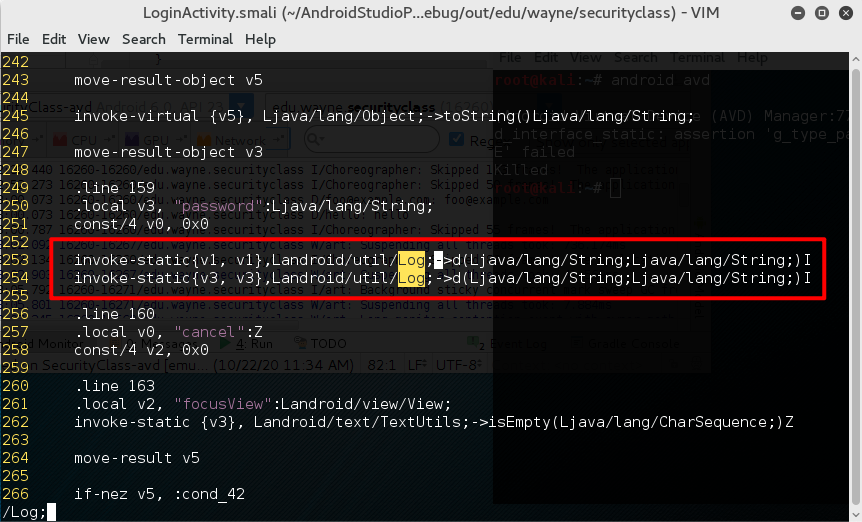
\includegraphics[width=0.95\textwidth]{img/pic2.png}
      \caption{code we added}
    \end{figure}

  \section{Turn in a screenshot of the captured username and password}

    \begin{figure}[H]
      \centering
      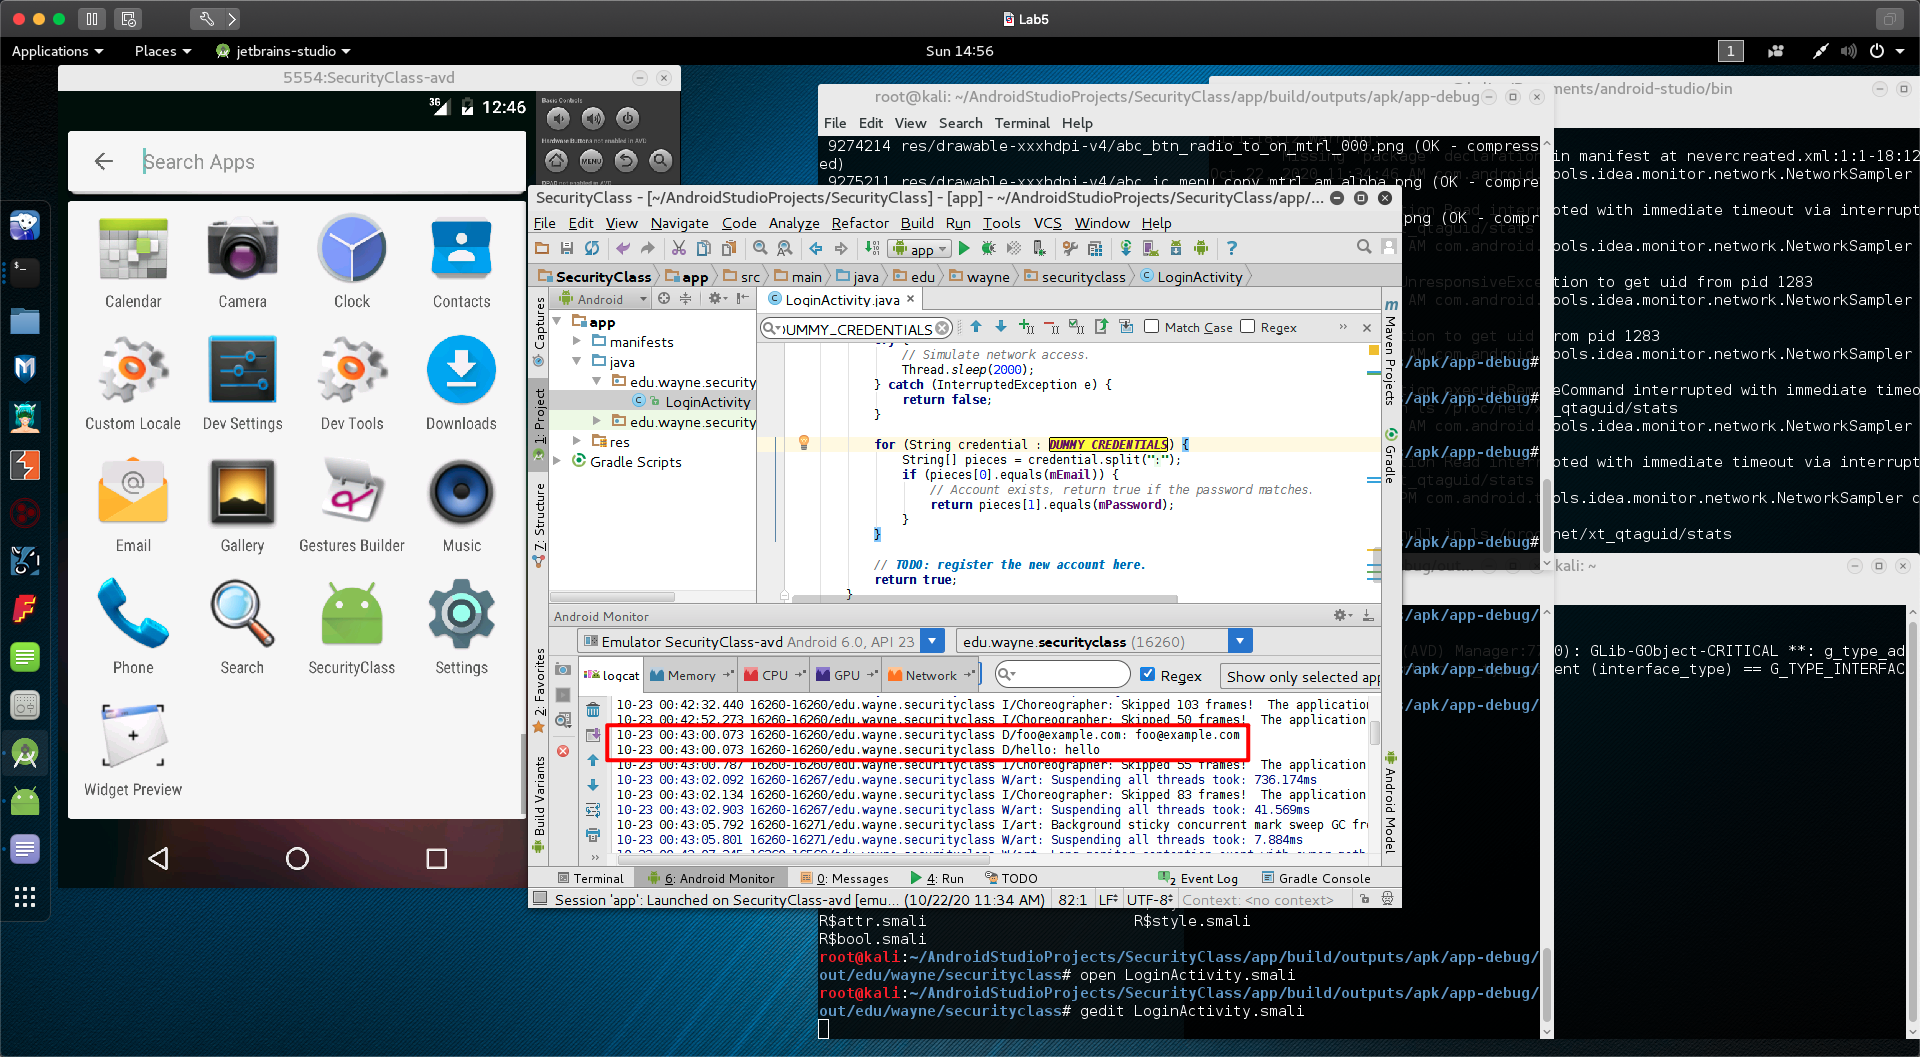
\includegraphics[width=0.95\textwidth]{img/pic1.png}
      \caption{username and password}
    \end{figure}

  \section{Describe the process to obfuscate an Android Application}

  ProGuard is a Java class file shrinker, optimizer, obfuscator, and preverifier. The shrinking step detects and removes unused classes, fields, methods, and attributes. The optimization step analyzes and optimizes the bytecode of the methods. The obfuscation step renames the remaining classes, fields, and methods using short meaningless names. These first steps make the code base smaller, more efficient, and harder to reverse-engineer. The final preverification step adds preverification information to the classes

    \subsection{What tools did you use?}

    ProGuard.

    \subsection{Can you still repackage the application using baksmali or smalitool? Justify your answer.}

    No, because we obfuscate the android application.

    \begin{figure}[H]
      \centering
      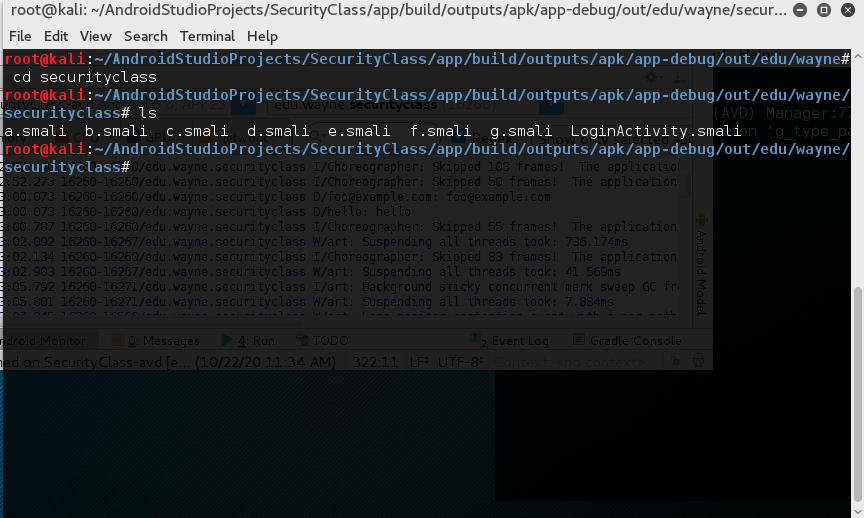
\includegraphics[width=0.95\textwidth]{img/pic3.png}
      \caption{obfuscate}
    \end{figure}

    \begin{figure}[H]
      \centering
      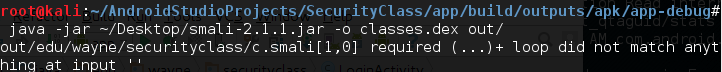
\includegraphics[width=0.95\textwidth]{img/pic4.png}
      \caption{repackage fail}
    \end{figure}
  
\end{document}
